\documentclass[11pt,a4paper,1p,sort&compress]{elsarticle}
\usepackage[utf8]{inputenc}
\usepackage[]{times}
\usepackage{fullpage}
\addtolength{\textheight}{1cm}
\usepackage{graphicx}
\usepackage{subfigure}
\usepackage{amsmath}
\usepackage{fancyhdr}

% TODO comment this to remove label
\usepackage{showkeys}

\date{}%leave empty

%\biboptions{longnamesfirst,angle,semicolon}
\usepackage{bm}
%% The amssymb package provides various useful mathematical symbols
\usepackage{amsfonts,amsmath,amssymb,amsthm}
%% The amsthm package provides extended theorem environments
%% \usepackage{amsthm}
\newtheorem{proposition}{Proposition}
\newtheorem{conjecture}{Conjecture}

\usepackage{tikz}
%\usepackage{pgfplots}
%\usepackage{pgfplotstable}
\usepackage{multicol}
\usepackage{multirow}

\usepackage{graphicx}
\usepackage{subfigure}
\usepackage{wrapfig}
\usepackage{float}

\usepackage[colorinlistoftodos]{todonotes}
%\usepackage[disable]{todonotes}

\journal{HAL}
\begin{document}

%--------------------------------------------------------------------------------
% HEADER
%--------------------------------------------------------------------------------
\begin{frontmatter}

%\title{Calcul de matrice d’impédance pour la simulation
%numérique des lignes de transmission multi-conducteur.}

\title{Impedance matrix computation for the numerical simulation of
multi-conductor transmission lines}

% TODO A COMPLETER
\author[ad1]{S. Asmar}
\ead{}
\author[ad2]{G. Dollé}
\ead{gdolle@unistra.fr}
\author[ad3]{J. Aghili}
\ead{jaghili@univ-montp2.fr}
\author[ad2]{N. Pham}
\ead{pham@math.unistra.fr}
\author[ad4]{A. Samaké}
\ead{}

\address[ad1]{Disneyland, Paris}
\address[ad2]{Université de Strasbourg / CNRS, IRMA / UMR  7501. Strasbourg, F-67000, France}
\address[ad3]{Université de Montpellier 2 / 34057 Montpellier Cedex 5, France}
\address[ad4]{Université de Grenoble 1 / CNRS, Laboratoire Jean Kuntzmann / UMR 5224, Grenoble, F-38041, France}

%\cortext[cor]{Autheur correspondant ??}

\begin{abstract}
  \input{chapters/abstract}
\end{abstract}

\begin{keyword}
  SEME 2014 Axessim Strasbourg
\end{keyword}

\end{frontmatter}

%--------------------------------------------------------------------------------
% HEADER
%--------------------------------------------------------------------------------

\section*{Introduction}
\label{sec:Introdution}
In this paper we are interested in  $N+1$ circular conductors
$\{w_i\}_{i=0,..,N}$, considered in the $x,y$-plane, with respective radii
$\{r_i\}_{i=0,..,N}$ and centers $\{X_i\}_{i=0,..,N}$. We mean by conductor
\todo{figure?} , either a cable or a set of cables traveled by an electric
\todo{a ameliorer ?} current in the $z$-axis, perpendicular to the plane. The
top conductor $w_0$ is to be thought as the largest armour containing all the
other conductors $w_i \, (i \ne 0)$. When the current travels over the cables,
the transmission model allow us to determine the coupling between the cables.
The model is a set of differential equations where the unknowns are the
intensity $U(t,z)$ and the electric current $I(t,z)$, functions of time and
space. The quantities are linked with coupling matrices $C$ and $L$ who has to
respect properties such as positiveness and symmetry according to the physics.
The main point of this paper is to analyse such behaviour at the numerical
scale and propose a way to compute those matrices. 


%%% Local Variables:
%%% mode: latex
%%% TeX-master: "../report"
%%% End:


\section*{The Physical model}
\label{sec:Model}
 %%%%%%%%%%%%%%%%
 % Useful stuff %
 %%%%%%%%%%%%%%%%
\renewcommand{\vec}[1]{\ensuremath{\mathbf #1}}

\subsection*{The governing equation}
\todo[inline]{from helluy's doc}
The transmission model line is given by the following system of differential equations
\begin{equation}
  \label{eq:model}
    \begin{array}{ccc}
      \partial_z U&=& L\partial_t I + RI \\
      \partial_z I&=& C\partial_t U + GU \\
    \end{array}
\end{equation}

where we denoted the following square matrices:
\begin{itemize}
\item  $L$ the inductance, required to be \textbf{definite-positive and symmetric}
\item $C$ the capacity, defined as the inverse of $L$, required to be \textbf{definite positive and symmetric}
\item $R$ the resistance\todo{pas sur du mot}, assumed to be diagonal
\item $G$ the conductancy, defined as the inverse of $R$.
\end{itemize}

we get rid \todo{change this} of the time dependancy in $\eqref{eq:model}$ by applying a Fourier transformation $(U,I) \mapsto (\hat{U},\hat{I})$, one finally gets, after dropping the hats the following system
\begin{equation}
  \label{eq:model.fourier}
    \begin{array}{ccc}
      \partial_z U &=& (j\omega L + R) I \\
      \partial_z I &=& (j\omega C  + G) U \\  
    \end{array}
\end{equation}
for the latter we denote by $Z$ the impedance matrix defined by $Z=(j\omega L + R)$ and $Y=(j\omega C  + G)$. The main concern of this paper is to compute $L$ with desired properties, independantly \todo{ ? } from the number of conductors, $C$ is straightforwardly deduced.

In the following chapters, we give the steps to compute the matrices at the continuous scale. We then suggest a way to enforce the symmetry and the definite positive conditions.
\subsection*{The single armour case}
\todo[inline]{rewrite from helluy's doc all the blabla}
In what follows we derive the expression of $C$ in the case of one armour $w_0$ containing $N$ cables $\{ w_i \}_{i=1,...,N}$. We assume that the magnetic field $\vec{B}$ derives from a potential field $\vec{A}=(0,0,\varphi(x,y))$ such that 
\[
\label{def:B}
\vec{B} = \rot  \vec{A}
\]

We focus on every $w_i$ inside $w_0$, the latter definiton combined with Maxwell-flux equation $\rot \vec{B} = \vec{j}$ on $w_i$ leads to a Poisson-like equation satisfied by $\varphi$ on $w_i$,

\begin{equation}
\label{eq:poissonwi}
\rot \vec{B} = -\Delta \varphi = j_z \quad \text{on } w_i
\end{equation}

Since $\varphi$ is assumed regular enough, one can use the Gauss identity to infer
\begin{equation}
  \label{eq:traceeqn}
  \begin{array}{rcl}
    \int_{w_i} (-\Delta \varphi) \, dV &=& \int_{w_i} (- \divg (\nabla \varphi))  dV \\
                                       &=& \int_{\partial w_i} (-\nabla\varphi \cdot \vec{n}) dS \\
                                       &=& \int_{\partial w_i} \nabla\varphi \cdot (-\vec{n})  \, dS \\
                                       &=& \int_{ \partial w_i} \nabla\varphi^{\text{ext}} \cdot (\vec{n}_i)  \, dS \\
                                       &=& I_i \\
  \end{array}
\end{equation}
where $\vec{n}_i$ denotes the normal vector pointing outside of $w_i$, $I_i=\int_{w_i}j_z$ the current along $w_i$ and since $\varphi$ is zero near the interior boundary, we consider it's  exterior contribution $\varphi^{\text{ext}}$ for the . The same computation holds for $w_0$, 

\begin{equation}
  \label{eq:traceeqnw0}
  \begin{array}{rcl}
    \int_{w_0} (-\Delta \varphi) \, dV &=& \sum_{k=1}^N \int_{w_k} (-\Delta \varphi) \, dV \\
                                      &=& \sum_{k=1}^N I_k \\
                                      &=& \int_{\partial w_0} \nabla \varphi \cdot \vec{n}_i dS \\
                                      &=& \int_{\partial w_0} \nabla \varphi^{\text{int}} \cdot \vec{n}_i dS \\
  \end{array}
\end{equation}
where $\varphi^{\text{int}}$ is the interior contribution of $\varphi$ in $w_0$. One set $\vec{I}=(I_1,...,I_N)$ the vector containing all the currents. One suppose that $\varphi$ is constant on each $w_i$ with value $\Phi_i$, one set the corresponding vector $\mathbf{\Phi}=(\Phi_1,...,\Phi_N)$. One wants to link $\mathbf{\Phi}$ to $\mathbf{I}$ by a linear relation. Thus, we introduce a family of smooth functions $\{ \zeta_j \}_{j=1...N}$ such that $\zeta_j = 1 $ on $w_j$ and 0 on $\cup_{\substack{k=1 \\ k\ne j}}^N w_k$. Since $\varphi$ is suppposed smooth, we suppose that $\varphi = \sum_{j=1}^N \Phi_j \zeta_j$.
\begin{equation}
  \label{eq:derive.cap}
  \begin{array}{rcl}
    \int_{w_i} (-\Delta \varphi)  &=& \int_{w_i} (- \sum_j \Phi_j \Delta \zeta_j) \\
                                  &=& \sum_j \Phi_j \left( \int_{\partial w_i} \nabla \zeta^{\text{ext}}_j \cdot \vec{n}_i \, dS \right) \\
                                  &=& I_i \\
  \end{array}
\end{equation}
for $1\le i \le N$,  we then get the relation 
\[
\mathbf{I} = M \mathbf{\Phi}
\]
where $M$ is defined trought it's coefficients $M_{ij}=\int_{\partial w_i} \nabla \zeta^{\text{ext}}_j \cdot \vec{n}_i \, dS$ where $1\le i,j \le N$. From this definition of $M$ we perform numerical tests in order to detect at which stage the lack of symmetry/definite-positiveness occurs.

\subsubsection*{Numerical tests}
We first reproduce the problem in a simple case. We consider a disk-shaped mesh with 6 disk holes placed at the same distance each from others. 

\begin{figure}[!h]
  \centering
  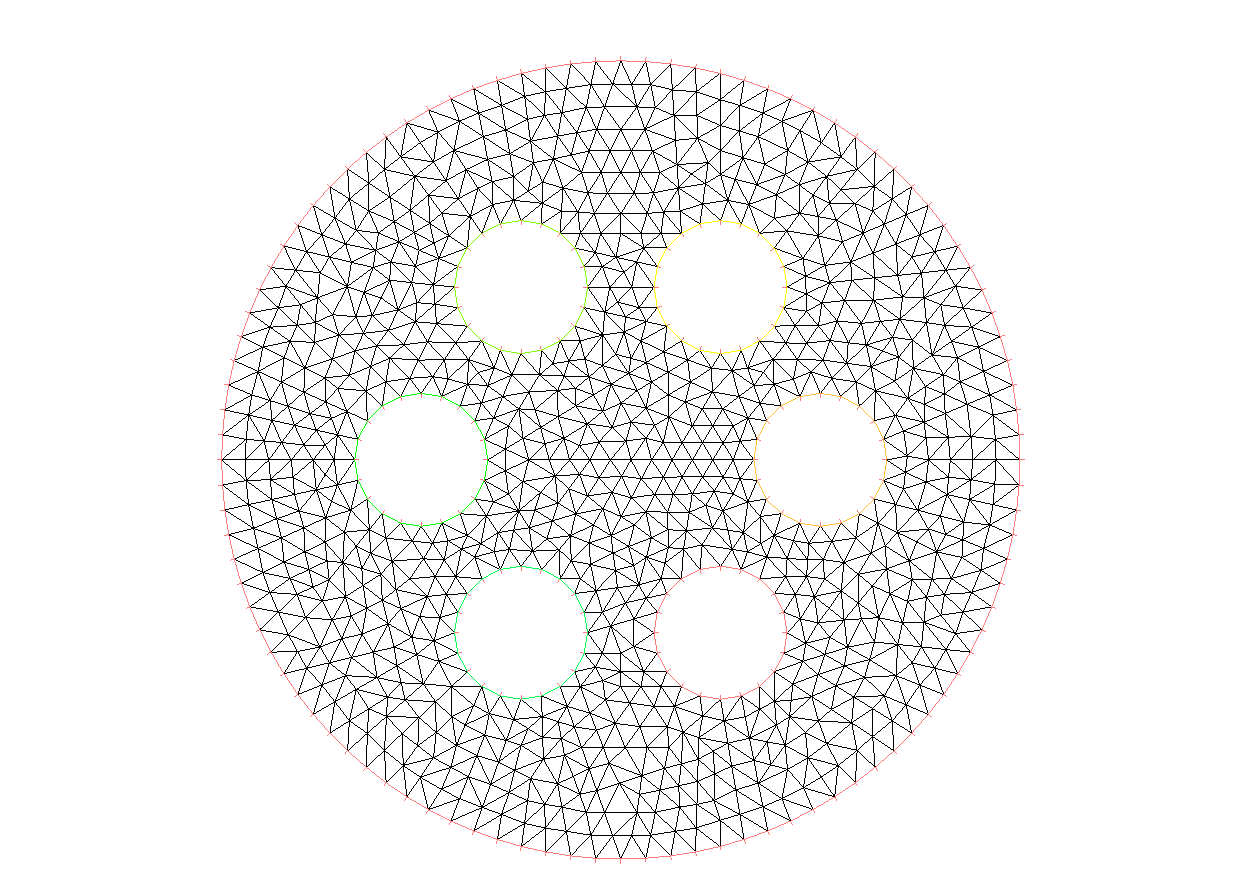
\includegraphics[scale=0.25]{fig/mesh_10.pdf}
  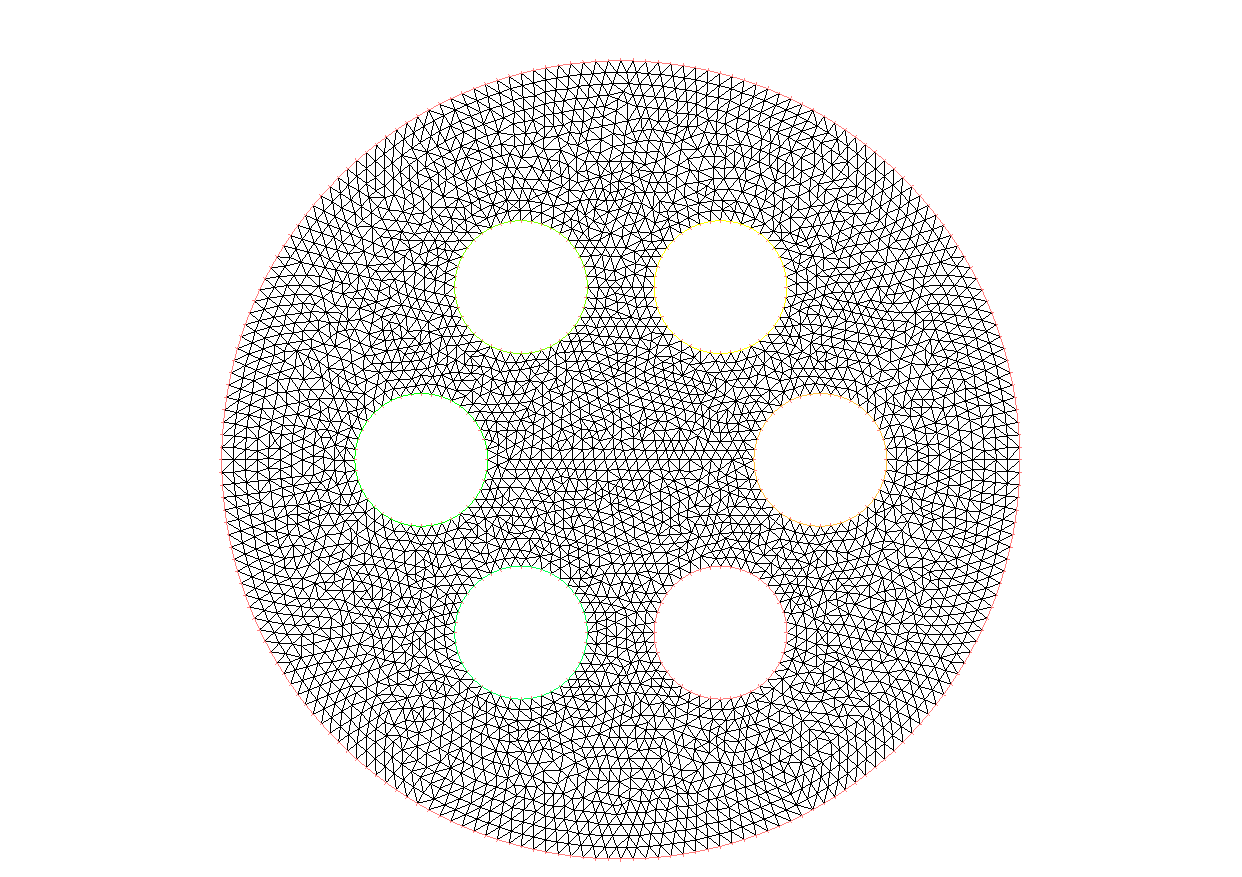
\includegraphics[scale=0.25]{fig/mesh_20.pdf}
  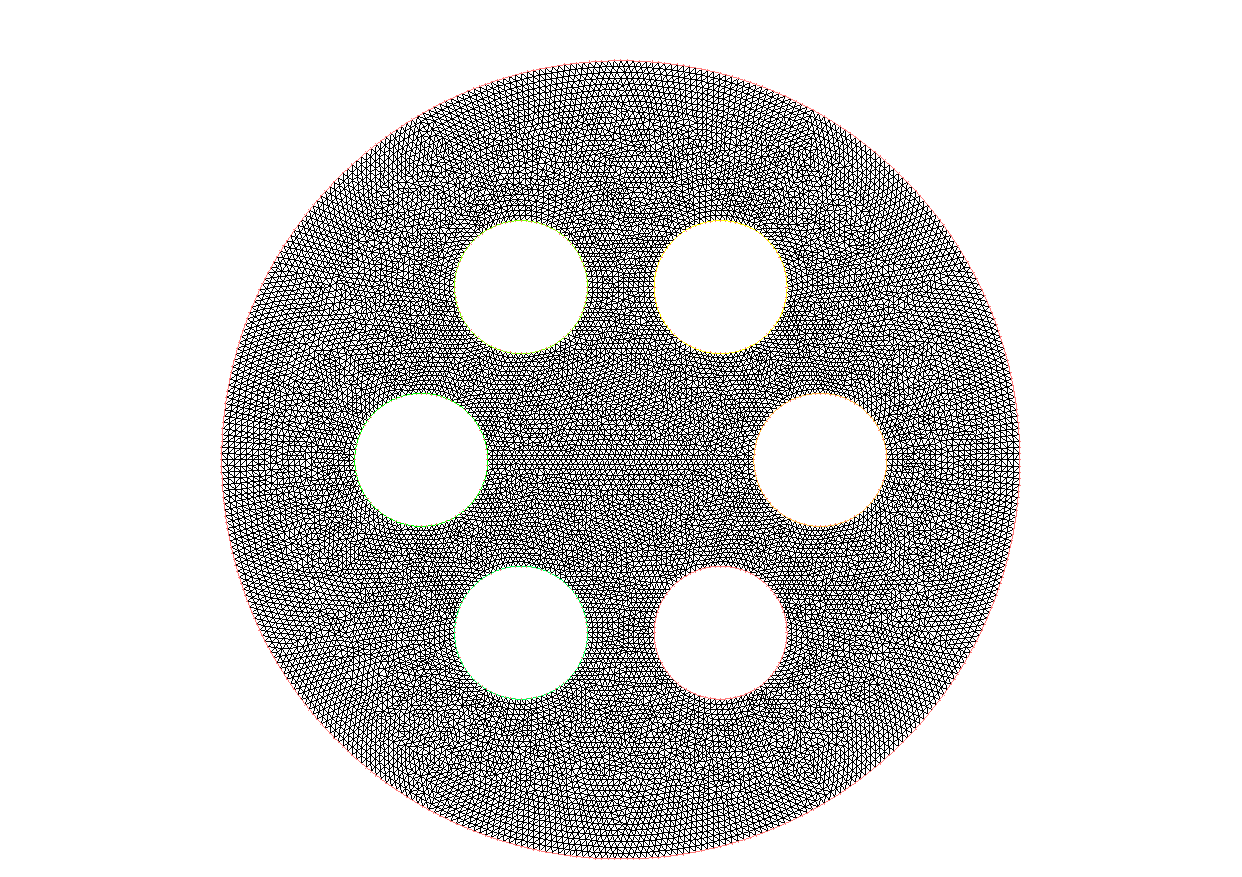
\includegraphics[scale=0.25]{fig/mesh_40.pdf}
  \caption{Mesh family used to compute $M$}
\label{fig:meshfamily}
\end{figure}



Since the coefficients $M_{ij}$ are computed according to a line integral, we first test the lack of symmetry versus the smallness \todo{a ameliorer} of the meshsize. The lack of symmetry is measured by estimating $|| M-M^T ||_\infty$. The following figure describe the evolution of the error when the mesh size is decreasing.


\begin{figure}[h]
  \centering
  \begin{tikzpicture}
    \pgfplotsset{width=0.95\textwidth, height=0.4\textwidth}
    \begin{semilogyaxis}[
      ymin=0,
      ymajorgrids=true, % grid=minor pour avoir tous les traits
      xlabel={Mesh size},
      ylabel={$|| M-M^T ||_{\infty}$},
      legend entries={
        Symmetry lack
      },
      legend style={legend pos=north west}
      ]
      \addplot [cyan,thick] table [x index=0,y index=1] {dat/err.dat};
    \end{semilogyaxis}
  \end{tikzpicture}
  \caption{Lack of Symmetry vs mesh size}
\label{fig:symm}
\end{figure}


 
\subsection*{The multiple armour/cable case}
\todo[inline]{rewrite from helluy's doc all the blabla}

\subsection*{Symmetry enforcement by weak formulation}


%%% Local Variables:
%%% mode: latex
%%% TeX-master: "../report"
%%% End:


\section*{Numerical results}
\label{sec:Results}
\subsection*{Impacts of the nonsymmetry}

\subsection*{Numerical tests}
%%% Local Variables:
%%% mode: latex
%%% TeX-master: "../report"
%%% End:


\section*{Conclusion}
\label{sec:Conclusion}
\input{chapters/conclusion}

\section*{Acknowledgments}
\label{sec:Acknowledgments}
\todo[inline]{Remercier team SEME, en particulier P. Helluy}
\section*{References}
\label{sec:References}
duplicate ?

\bibliographystyle{elsarticle-num}
\bibliography{seme2014_axessim}

\nocite{*}

\end{document}
%%% Local Variables:
%%% coding: utf-8
%%% mode: latex
%%% TeX-PDF-mode: t
%%% TeX-parse-self: t
%%% x-symbol-8bits: nil
%%% TeX-auto-regexp-list: TeX-auto-full-regexp-list
%%% TeX-master: t
%%% ispell-local-dictionary: "american"
%%% End:
